\documentclass[tikz,dvipsnames]{standalone}

\usepackage[]{xcolor}
\PassOptionsToPackage{dvipsnames}{xcolor}

\usetikzlibrary{calc}
\usetikzlibrary{decorations.pathmorphing,patterns,decorations.markings,arrows.meta,intersections}


\tikzset{
  cross/.style={
    path picture={
      \draw[thick]
        (path picture bounding box.south east) -- (path picture bounding box.north west)
        (path picture bounding box.south west) -- (path picture bounding box.north east);
    }
  }
}


\tikzset{
    angle bracket base/.style 2 args={
        to path={
            -- ($(\tikztostart)!0.5!(\tikztotarget)!#1!#2:(\tikztotarget)$) -- (\tikztotarget)
        }
    },
    angle bracket/.style={angle bracket base={#1}{90}},
    angle bracket/.default=0.4cm,
    angle bracket flipped/.style={angle bracket base={#1}{-90}},
    angle bracket flipped/.default=0.4cm
}

%set coordinates that randomly perturbes the original path
\tikzset{set random waves/.style args={#1and#2with name #3}{postaction={decorate,decoration={markings,
mark=at position 0.1 with {\coordinate[xshift={rand*#1},yshift={rand*#2}] (#3-1);},
mark=at position 0.2 with {\coordinate[xshift={rand*#1},yshift={rand*#2}] (#3-2);},
mark=at position 0.3 with {\coordinate[xshift={rand*#1},yshift={rand*#2}] (#3-3);},
mark=at position 0.4 with {\coordinate[xshift={rand*#1},yshift={rand*#2}] (#3-4);},
mark=at position 0.5 with {\coordinate[xshift={rand*#1},yshift={rand*#2}] (#3-5);},
mark=at position 0.6 with {\coordinate[xshift={rand*#1},yshift={rand*#2}] (#3-6);},
mark=at position 0.7 with {\coordinate[xshift={rand*#1},yshift={rand*#2}] (#3-7);},
mark=at position 0.8 with {\coordinate[xshift={rand*#1},yshift={rand*#2}] (#3-8);},
mark=at position 0.9 with {\coordinate[xshift={rand*#1},yshift={rand*#2}] (#3-9);}
}}}}


\tikzset{
arrow at/.style 2 args={postaction={decorate,decoration={
    markings,
    mark=at position #1 with {\arrow{Stealth[#2]}}
  }}},
}



\begin{document}
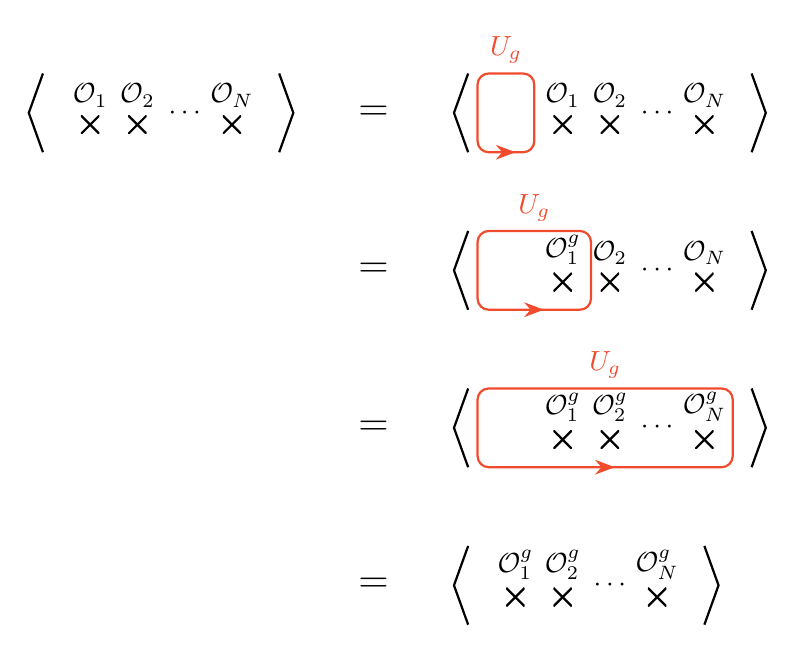
\begin{tikzpicture}[xscale=1.2]
\begin{scope}
% brackets
\draw[thick] (.5,-.5) to[angle bracket=.15cm] ++(0,1);
\draw[thick] (3,-.5) to[angle bracket flipped=.15cm] ++(0,1);

% operator insertions
\foreach \x[count=\xi] in {1,1.5,2.5} {
\coordinate (op-\xi) at (\x,-.15);
\node[cross, minimum size=1] at (op-\xi) {};
}
\node[anchor=south,yshift=.1cm] at (op-1) {$\mathcal{O}_1$};
\node[anchor=south,yshift=.1cm] at (op-2) {$\mathcal{O}_2$};
\node[anchor=south,yshift=.1cm] at (op-3) {$\mathcal{O}_N$};
\node at (2,0) {$\cdots$};

\end{scope}

\node at (4,0) {\Large $=$};

\begin{scope}[xshift=5cm]
% brackets
\draw[thick] (0,-.5) to[angle bracket=.15cm] ++(0,1);
\draw[thick] (3,-.5) to[angle bracket flipped=.15cm] ++(0,1);

% operator insertions
\foreach \x[count=\xi] in {1,1.5,2.5} {
\coordinate (op-\xi) at (\x,-.15);
\node[cross, minimum size=1] at (op-\xi) {};
}
\node[anchor=south,yshift=.1cm] at (op-1) {$\mathcal{O}_1$};
\node[anchor=south,yshift=.1cm] at (op-2) {$\mathcal{O}_2$};
\node[anchor=south,yshift=.1cm] at (op-3) {$\mathcal{O}_N$};
\node at (2,0) {$\cdots$};

\draw[thick,RedOrange,rounded corners] (.1,-.5) rectangle (.7,.5);
\node[anchor=south,RedOrange] at (.4,.5) {$U_g$};
\node[rotate=-90] at (.4,-.5) {\tikz{\draw[-{Stealth[RedOrange,length=.25cm]}] (0,0)}};
%\path[arrow at={.5}{RedOrange}] (.1,-.5) -- (.7,-.5);

\end{scope}

\node at (4,-2) {\Large $=$};

\begin{scope}[xshift=5cm,yshift=-2cm]
% brackets
\draw[thick] (0,-.5) to[angle bracket=.15cm] ++(0,1);
\draw[thick] (3,-.5) to[angle bracket flipped=.15cm] ++(0,1);

% operator insertions
\foreach \x[count=\xi] in {1,1.5,2.5} {
\coordinate (op-\xi) at (\x,-.15);
\node[cross, minimum size=1] at (op-\xi) {};
}
\node[anchor=south,yshift=.1cm] at (op-1) {$\mathcal{O}_1^g$};
\node[anchor=south,yshift=.1cm] at (op-2) {$\mathcal{O}_2$};
\node[anchor=south,yshift=.1cm] at (op-3) {$\mathcal{O}_N$};
\node at (2,0) {$\cdots$};

\draw[thick,RedOrange,rounded corners] (.1,-.5) rectangle (1.3,.5);
\node[anchor=south,RedOrange] at (.7,.5) {$U_g$};
\node[rotate=-90] at (.7,-.5) {\tikz{\draw[-{Stealth[RedOrange,length=.25cm]}] (0,0)}};
%\path[arrow at={.5}{RedOrange}] (.1,-.5) -- (.7,-.5);
\end{scope}

\node at (4,-4) {\Large $=$};

\begin{scope}[xshift=5cm,yshift=-4cm]
% brackets
\draw[thick] (0,-.5) to[angle bracket=.15cm] ++(0,1);
\draw[thick] (3,-.5) to[angle bracket flipped=.15cm] ++(0,1);

% operator insertions
\foreach \x[count=\xi] in {1,1.5,2.5} {
\coordinate (op-\xi) at (\x,-.15);
\node[cross, minimum size=1] at (op-\xi) {};
}
\node[anchor=south,yshift=.1cm] at (op-1) {$\mathcal{O}_1^g$};
\node[anchor=south,yshift=.1cm] at (op-2) {$\mathcal{O}_2^g$};
\node[anchor=south,yshift=.1cm] at (op-3) {$\mathcal{O}_N^g$};
\node at (2,0) {$\cdots$};

\draw[thick,RedOrange,rounded corners] (.1,-.5) rectangle (2.8,.5);
\node[anchor=south,RedOrange] at (1.45,.5) {$U_g$};
\node[rotate=-90] at (1.45,-.5) {\tikz{\draw[-{Stealth[RedOrange,length=.25cm]}] (0,0)}};
%\path[arrow at={.5}{RedOrange}] (.1,-.5) -- (.7,-.5);

\end{scope}

\node at (4,-6) {\Large $=$};

\begin{scope}[xshift=4.5cm,yshift=-6cm]
% brackets
\draw[thick] (.5,-.5) to[angle bracket=.15cm] ++(0,1);
\draw[thick] (3,-.5) to[angle bracket flipped=.15cm] ++(0,1);

% operator insertions
\foreach \x[count=\xi] in {1,1.5,2.5} {
\coordinate (op-\xi) at (\x,-.15);
\node[cross, minimum size=1] at (op-\xi) {};
}
\node[anchor=south,yshift=.1cm] at (op-1) {$\mathcal{O}_1^g$};
\node[anchor=south,yshift=.1cm] at (op-2) {$\mathcal{O}_2^g$};
\node[anchor=south,yshift=.1cm] at (op-3) {$\mathcal{O}_N^g$};
\node at (2,0) {$\cdots$};

%\path[arrow at={.5}{RedOrange}] (.1,-.5) -- (.7,-.5);

\end{scope}
    
\end{tikzpicture}
\end{document}
